\section{Изоморфизм и гомеоморфизм графов. Примеры изоморфных и гомеоморфных графов. Способы 
проверки изоморфизма графов. Инварианты графа. Дополнение графа, проверка изоморфизма 
графов с помощью дополнений. Выяснить, являются ли графы G1 и G2 изоморфными, 
гомеоморфными.}

\begin{definition}
    \textit{Изоморфизм графов} -- биективное отображение $\varphi: V_1 \rightarrow V_2$, такое что:
    \begin{align*}
        (\forall u,v \in V)((u,v) \in E_1) \Leftrightarrow (\varphi(u),\varphi(v)) \in E_2
    \end{align*}
\end{definition}

Изоморфные графы обозначаются: $G_1 \cong G_2$

Изоморфные объекты \textit{не различимы} с точки зрения математики. Это экземпляры
одного и того же математического объекта. Изоморфные объекты имеют одинаковое
число элементов и свойств.

Изоморфизм графов можно определить:
\begin{enumerate}[left=0.0em, labelsep=1em, topsep=0.0em, itemsep=0pt, parsep=0.5em]
    \item По определению (найдя биективное отображение множества вершин,
    сохраняющее смежность)
    \item Перерисовав один из графов так, чтобы изображение совпало с другим
    графом
    \item Сравнив матрицы смежности графов
\end{enumerate}

\begin{theorem}
    Графы изоморфны тогда и только тогда, когда матрицу смежности
одного из них можно получить из матрицы смежности другого путём
одновременной перестановки местами $i$-ой и $j$-ой строк и столбцов.
\end{theorem}

Пример изоморфных графов:
\begin{figure}[h]
    \centering
    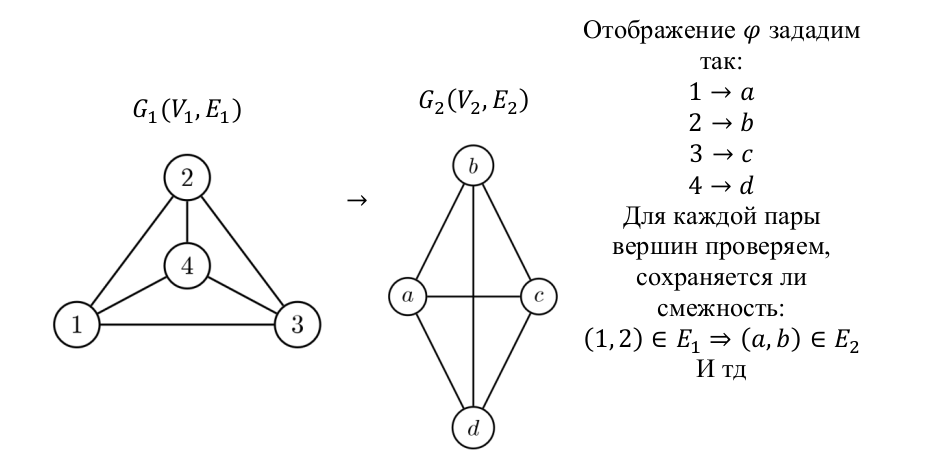
\includegraphics[scale=0.25]{3_iso.png}
\end{figure}

\begin{definition}
    \textit{Инвариантом изоморфизма графов} называется некоторое
    (обычно числовое) значение или упорядоченный набор значений,
    характеризующий структуру графа и не зависящий от способа его задания.
\end{definition}

Инвариантами графа являются:
\begin{enumerate}[left=0.0em, labelsep=1em, topsep=0.0em, itemsep=0pt, parsep=0.5em]
    \item Количество вершин
    \item Количество ребер
    \item Набор степеней вершин (упорядоченный)
    \item Определитель матрицы смежности
    \item Количество компонент связности
    \item Хроматическое число и т.д.
\end{enumerate}

Пусть $G(V,E)$ -- простой неориентированный граф.

\begin{definition}
    Дополнением графа $G$ называется граф $\overline{G}(\overline{V},\overline{E})$,
    у которого $\overline{V}=V$, в множестве $\overline{E}$ содержатся ребра полного графа,
    которых нет в множестве $E$.
\end{definition}

\begin{theorem}
    Простые графы $G$ и $H$ изоморфны тогда и только тогда, когда изоморфны их дополнения.
    \begin{align*}
        G \cong H \Leftrightarrow \overline{G} \cong \overline{H}
    \end{align*}
\end{theorem}

\begin{definition}
    Граф является самодополнительным, если он изоморфен своему дополнению.
\end{definition}

Понятие изоморфизма можно дать и для произвольных графов.

\begin{definition}
    Граф $G_1(V_1,E_1)$ и $G_2(V_2,E_2)$ \textit{изоморфны}, если $\exists$
    биективные отображения $\varphi : V_1 \rightarrow V_2$ и $h: E_1 \rightarrow E_2$
    такие, что:
    $$e = (u,v) \in E_1 \Leftrightarrow h(e) = (\varphi(u),\varphi(v)) \in E_2$$
\end{definition}